\documentclass[12pt]{article}

\usepackage[paper=letterpaper, margin=0.5in, footskip=0.25in]{geometry}
\usepackage{amsmath}
\usepackage{datetime}
\usepackage{amssymb}
\usepackage{titlesec}
\usepackage{enumitem}
\usepackage{graphicx}
\usepackage{hyperref}
\usepackage[skip=0.15em]{caption}
\usepackage[font=normal]{subfig}
\usepackage{framed}

\newdateformat{monthyeardate}{\monthname[\THEMONTH] \THEYEAR}

\makeatletter
\def\@maketitle{
  \newpage
  \vspace*{-\topskip}
  \begingroup\centering
  \let \footnote \thanks
  \hrule height \z@
    {\fontsize{16}{19.2} \@title \par}
    \vskip 0.25em 
    {\large
      \lineskip 0.5em 
      \begin{tabular}[t]{c}
        \@author
      \end{tabular}\par}
    \vskip 0.25em 
    {\large \monthyeardate\today}
  \par\endgroup
  \vskip 1em
}
\makeatother

\titleformat{\section}{\normalfont\scshape}{\textbf\thesection}{0em{\textbf{ – }}}{\textbf}
\titleformat{\subsection}{\normalfont\scshape}{\textit\thesubsection}{0em{\textit{ – }}}{\textit}
\titlespacing*{\section}{0pt}{1.5em}{0.5em}
\titlespacing*{\subsection}{0pt}{1em}{0.33em}

\title{\textbf{Soldering Guide}}
\author{Erk Sampat}
\begin{document}
\maketitle

\begin{center}
    Instructional Lab Group \\
    UC Santa Barbara Department of Physics
\end{center}

\section{Theory}
\subsection{Introduction}
Soldering is the process of melting a metal with a hot iron and allowing the molten metal to flow onto two or more different pieces of metal and harden, joining them together. The goal is to create neat, reliable joints. We are going to cover soldering through-hole components by hand. Learning the information in this section is NOT necessary, but it helps tremendously to know what is actually going on.

\subsection{Metals Joined Together}
For electronics, the metals being joined/soldered together are typically made of copper. For example, you may want to solder the pins of an LED to a copper strip on a perf-board. (Some wires and pins of electronic components will appear silver because they are already coated in solder, but underneath they are usually made of copper.)

\subsection{Metal that is Melted}
The metal being melted – called the solder – usually contains little to no copper because copper’s melting point is much too high for practical use. Instead, we use alloys that contain mixtures of lead, tin, bismuth, silver, and sometimes a little copper. Leaded solder often follows the Sn63/Pb37 (63\% tin, 37\% lead) formula; unleaded formulas vary. Generally, leaded solder is easier to work with, but it carries the obvious risk of containing lead. Solder primarily comes in a spool of soft, silver-looking wire, but other forms like paste exist for special processes. We will focus on soldering with standard wire solder. Wire solder comes in various thicknesses, but for general use, around 0.4mm is recommended.
\begin{figure}[h]
    \caption{a spool of 0.38mm 63/37 leaded solder.}
    \centering 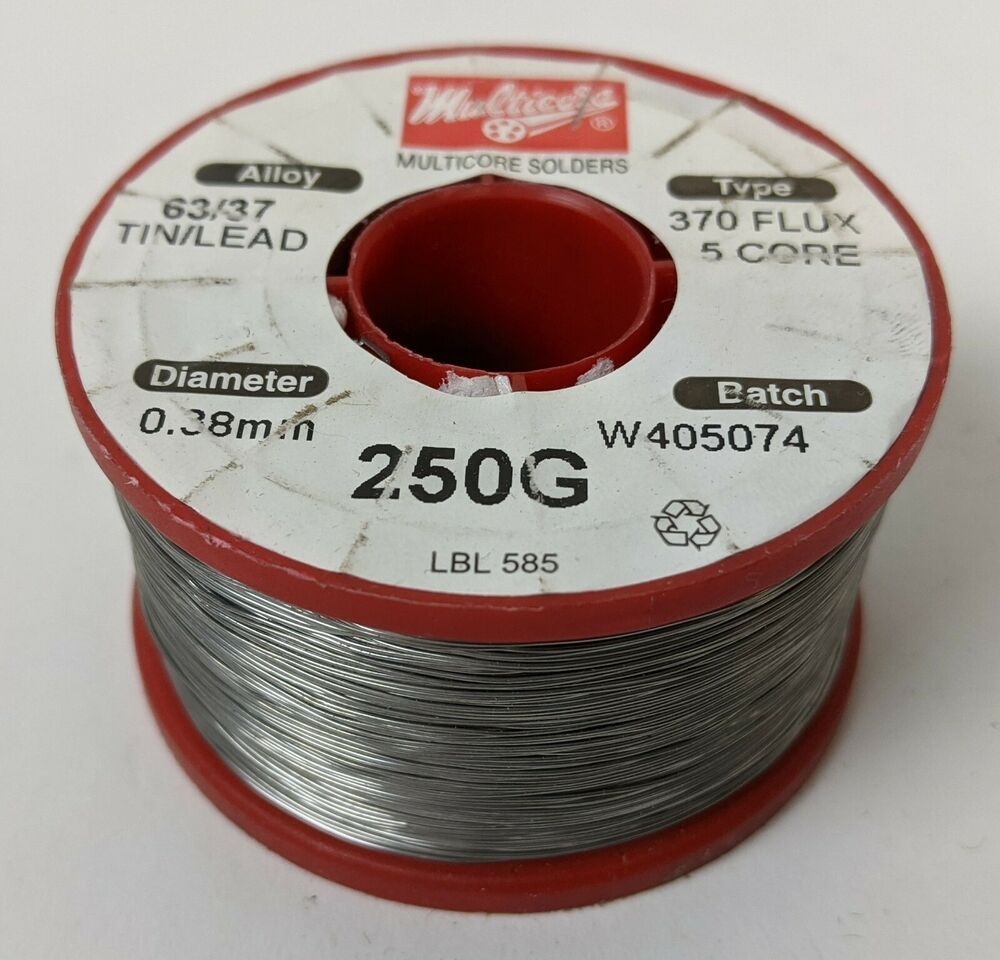
\includegraphics[scale=0.25]{images/solder_spool.jpg}
\end{figure}

\pagebreak

\subsection{Oxides; Flux}
Copper oxidizes easily, which is a problem. Molten solder will not adhere to copper that is coated in a layer of oxide. To solve this, nearly every solder will contain flux, which is usually made of rosin. You may hear the term ``rosin-core solder,'' which means that at the core of the wire of solder is a thin strand of rosin wax. When the hot iron melts the solder, the flux melts along with it. The liquid flux dissolves the oxides, leaving a fresh surface of copper for the molten solder to adhere to. In essence, \emph{flux is what allows solder to flow.} However, the flux won’t remain there forever – it will evaporate or burn off within a few seconds. This is what causes the fumes you see when soldering. It is a \emph{myth} that these fumes contain lead; the temperatures are far too low to vaporize any metals. For this reason, leaded solder is not particularly dangerous to work with as long as you wash your hands after you’re done. Regardless, inhaling flux fumes is still not good for you, and a fan or fume extractor is recommended (especially in areas with poor ventilation).
\begin{figure}[h]
    \caption{flux dissolves the oxide layer, allowing solder to bond with the base metal.}
    \centering 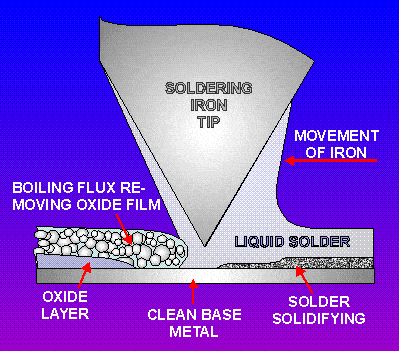
\includegraphics[scale=0.75]{images/oxidation_diagram.jpg}
\end{figure}

\subsection{Adding Extra Flux}
Sometimes, extra flux can be added directly when soldering a joint. This flux can come in a variety of forms, but the most common are pens, gels, and pastes. The principle when using any of these is the same: apply flux to the metals being soldered before applying heat. While adding extra flux can be helpful in certain situations, it is easy to add too much. With good quality solder, equipment, and technique, extra flux should rarely be needed.
\begin{figure}[h]
    \caption{different types of flux – [a] paste, [b] gel, and [c] pen.}
    \centering
    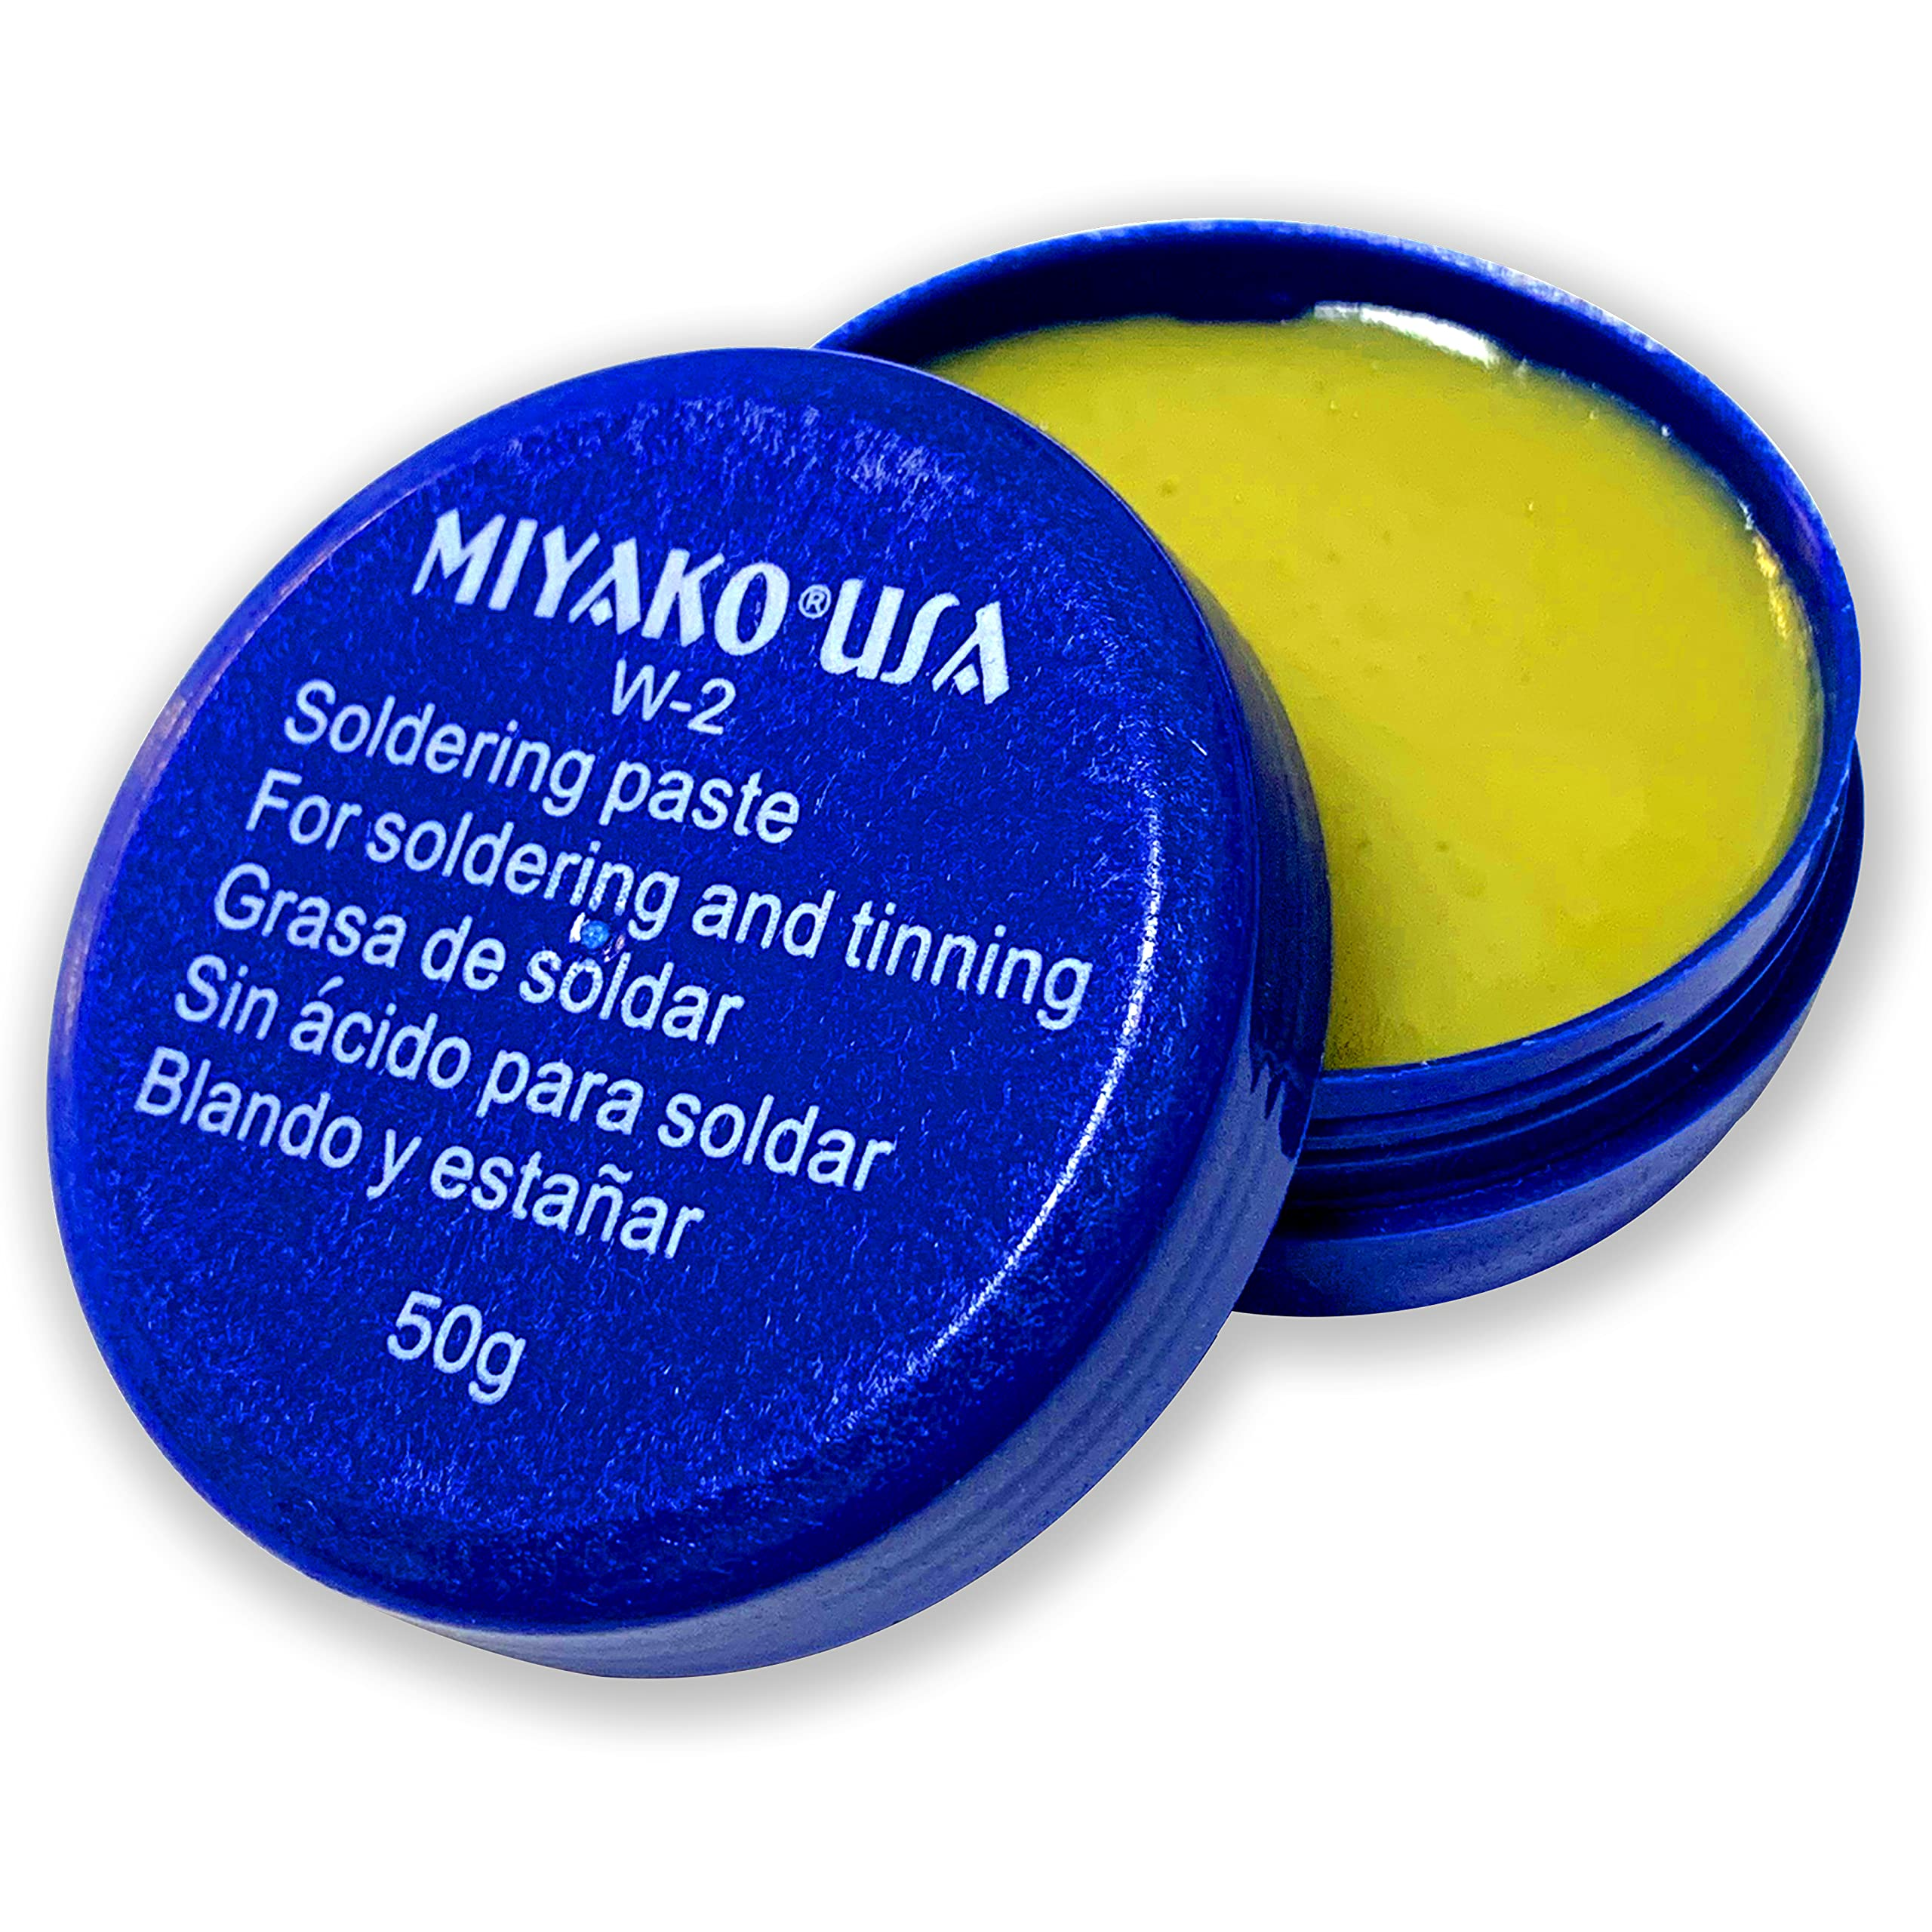
\includegraphics[scale=0.04]{images/flux_paste.jpg}
    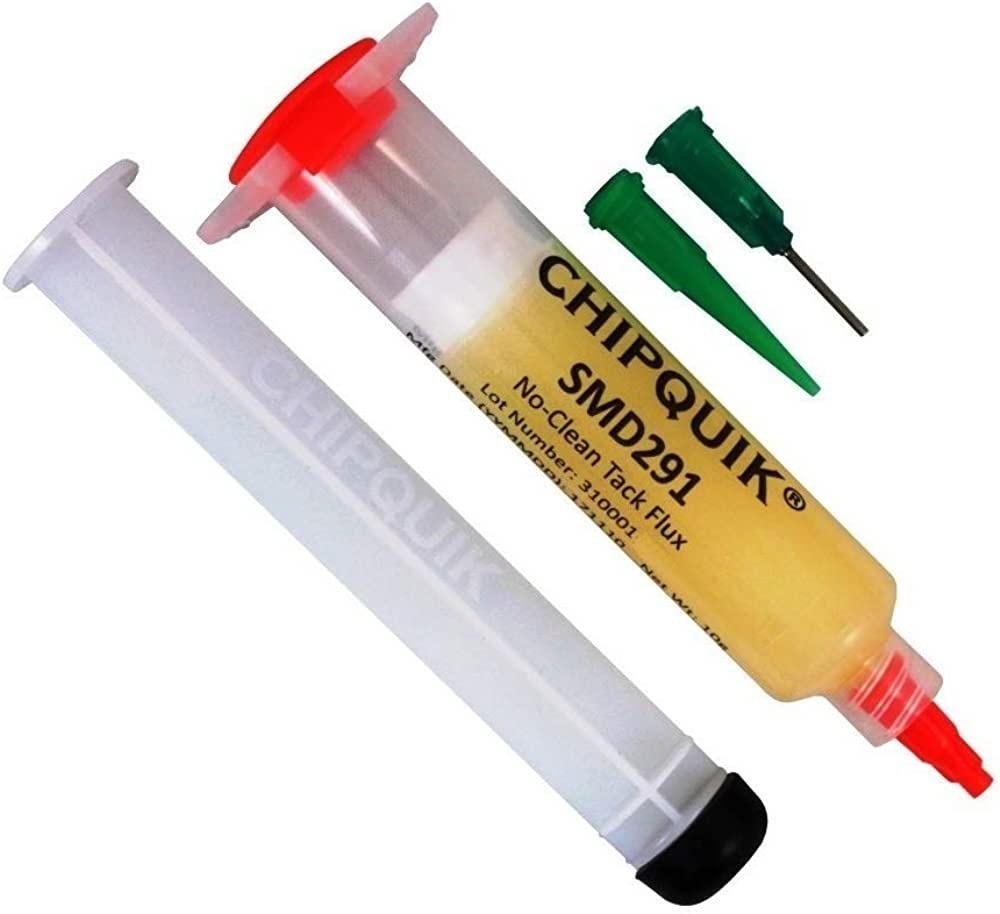
\includegraphics[scale=0.1]{images/flux_gel.jpg}
    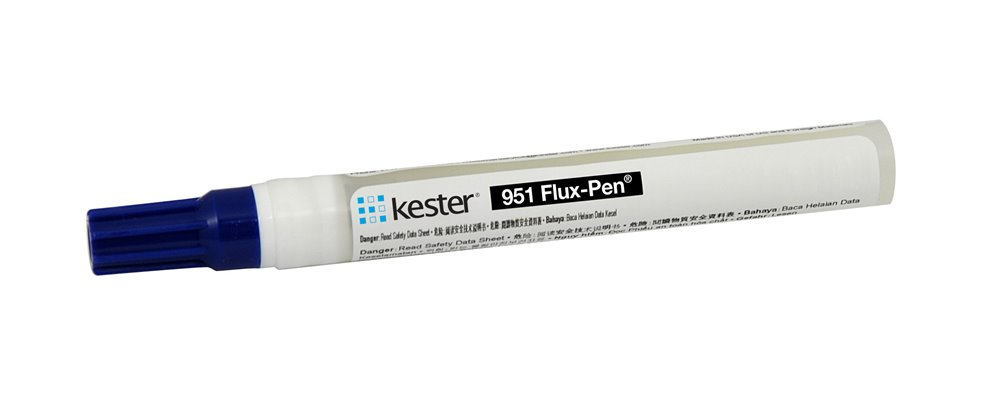
\includegraphics[scale=0.2]{images/flux_pen.jpg}
\end{figure}

\subsection{Soldering Tip – Composition}
Molten solder will always flow towards what is hot. So if the soldering tip is hot, why doesn't the solder stick to it and never flow elsewhere? Tips are specifically made to prevent this. On the inside, they are mostly copper because copper is a good heat conductor. However, solder adheres to copper much too strongly. To combat this, the outside of the tip is coated in a very thin layer of iron. Solder does stick to iron to some extent – otherwise the tip would be useless – but solder readily flows off of iron when something more preferential (like copper) is available. Why not make the entire tip out of iron, then? Iron does not conduct heat nearly as well as copper does, so it would be extremely inefficient.
\begin{figure}[h]
    \caption{anatomy of a soldering tip.}
    \centering 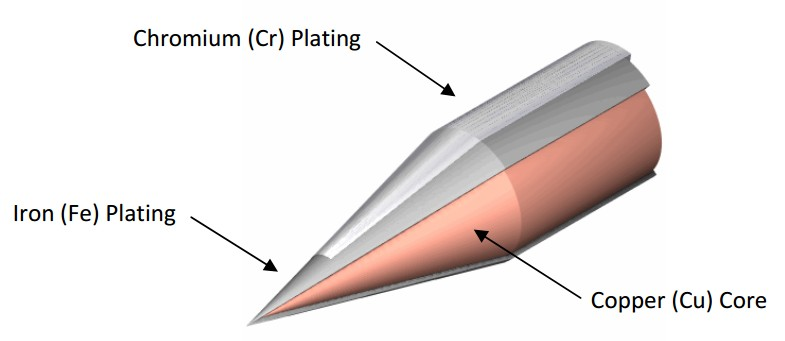
\includegraphics[scale=0.75]{images/tip_anatomy.jpg}
\end{figure}

\subsection{Tip Care}
Because the tip is coated in this thin layer of iron, care must be taken to prolong tip life. Taking good care of a tip can yield years of service, while failing to do so can destroy a tip in a matter of days. There are two primary causes of damage to a tip: oxidation of the iron coating and erosion of the iron coating. To avoid eroding the iron coating, use a brass wire nest designed specifically for soldering irons to clean the tip. Do NOT use a wet sponge, and do not clean the tip excessively or aggressively. Also, refrain from scraping or pushing any pins with the tip. To prevent oxidation, do not use excessive heat (discussed later), and \emph{always keep solder on the tip.} That is, before you put the iron in its stand temporarily, melt a little extra solder on the tip. Before you turn the iron off, clean the tip and melt some fresh solder on it before it cools down. And again, do not use a wet sponge to clean the tip – the water will accelerate oxidation. A tip in good condition will appear shiny, while an oxidized tip will appear dull.
\begin{figure}
    \centering
    \begin{minipage}{0.5\textwidth}
        \centering
        \caption{a brass wire nest.}
        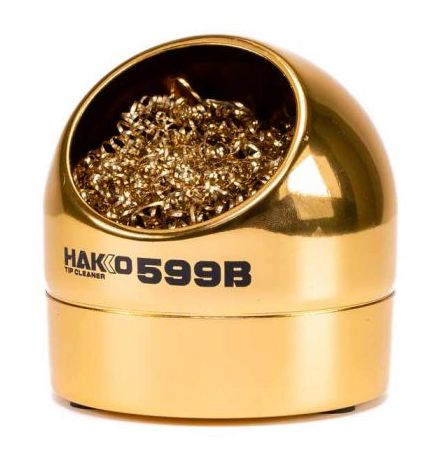
\includegraphics[scale=0.25]{images/tip_cleaner.jpg}
    \end{minipage}%
    \begin{minipage}{0.5\textwidth}
        \centering
        \caption{an oxidized tip struggling to take on solder.}
        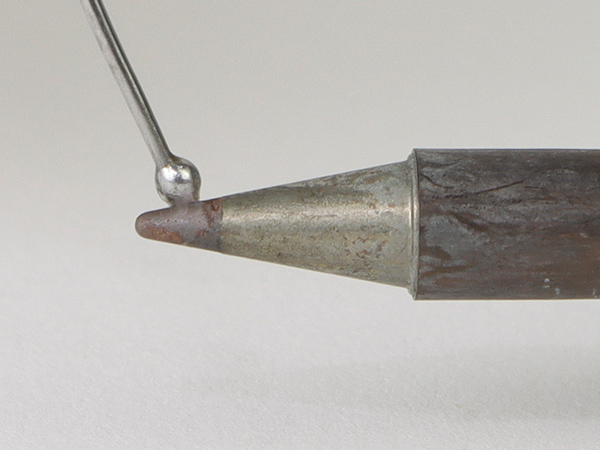
\includegraphics[scale=0.25]{images/oxidized_tip.jpg}
    \end{minipage}
\end{figure}

\subsection{Temperatures, Wattage, Thermal Mass; Tip Styles}
This is perhaps the most controversial aspect of soldering because everyone has their preferred temperature, iron, and tip style. However, there are guidelines. For temperature, 650°F is plenty for leaded solder. Unleaded solder often requires more. However, wattage and thermal mass come into play. Wattage is how much power the iron can dump into the tip as heat. If you have a really hot tip but the iron cannot supply much power, the heat from the tip will quickly get sucked away, and the iron will struggle to restore the tip temperature. This can be extremely frustrating, so an iron that can provide at least 50 watts of power is recommended (65 watts or above is ideal). Similarly, thermal mass plays a role. A large, heavy tip can hold more heat than a small, fine tip, so large tips are better for making big joints. Be careful with fine tips – using them on joints that are too large is difficult, as they cannot supply enough heat to melt all the solder. The solder will harden prematurely and the iron can become stuck to it. It is important to use an appropriate tip for the joint. Finally, the shape of the tip can make a difference as well. 1.6mm chisel tips are recommended for general soldering, as the flat sides allow for more area of contact between metals and the tip, increasing the efficiency of heat transfer. Some people prefer conical tips. It is best to start with a chisel tip, then experiment and decide what you like best.
\begin{figure}[h]
    \caption{[a] chisel tip, [b] conical tip.}
    \centering
    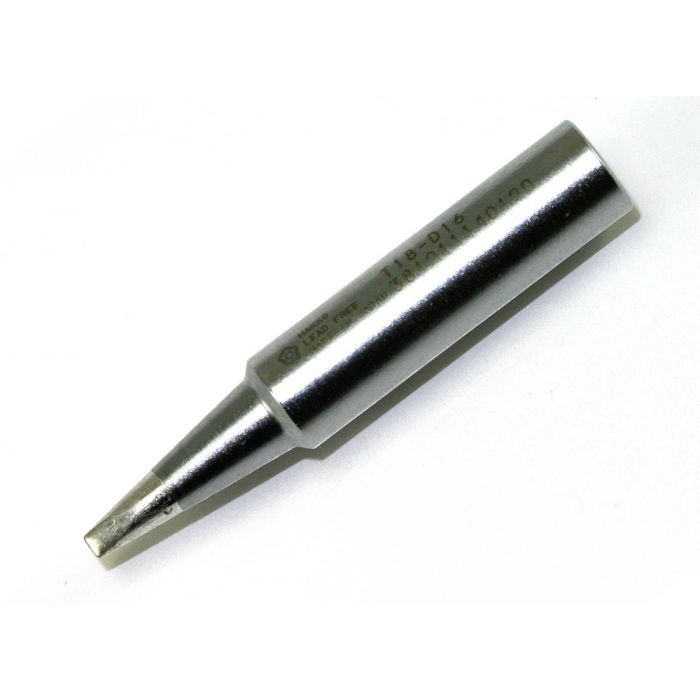
\includegraphics[scale=0.3]{images/chisel_tip.jpg}
    \hspace{0.125\textwidth}
    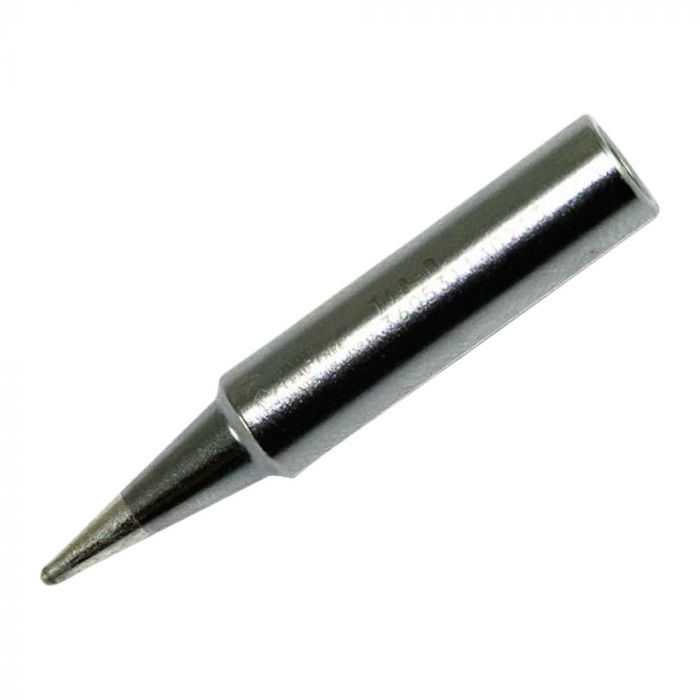
\includegraphics[scale=0.3]{images/conical_tip.jpg}
\end{figure}

\subsection{Conclusion}
We have examined the entire process of soldering by hand, moving from the metals being soldered all the way to the tip. Below, the steps to solder should make intuitive sense given all that we have discussed.

\pagebreak

\section{Steps}
\subsection{Adding Solder}
\begin{enumerate}
    \item Apply a little solder to the tip of a hot iron. Ensure that the tip becomes evenly coated in solder.
    \item Touch the metals that need to be soldered together with the tip. Let the metals heat up for a second or two (longer if there is a lot of metal mass).
    \item Begin feeding solder. Ideally, feed it such that it touches the hot tip as well as the metals being soldered together.
    \item Once a conical-shaped joint has formed, immediately stop adding solder. Adding excessive solder is a common error.
    \item Move the iron away from the joint. Give the joint a few seconds to cool and harden. Do not leave the iron on the joint for long after you stop feeding solder.
    \item Inspect the joint. It should be smooth and shiny. If it isn't, it is a ``cold joint'' and you need to touch it up. Repeat the process described above, but add very little additional solder. Alternatively, add flux.
    \item If there is too much solder on the joint, see \textit{Removing Solder} below.
\end{enumerate}
\begin{figure}[h]
    \caption{good vs. bad solder joints.}
    \centering 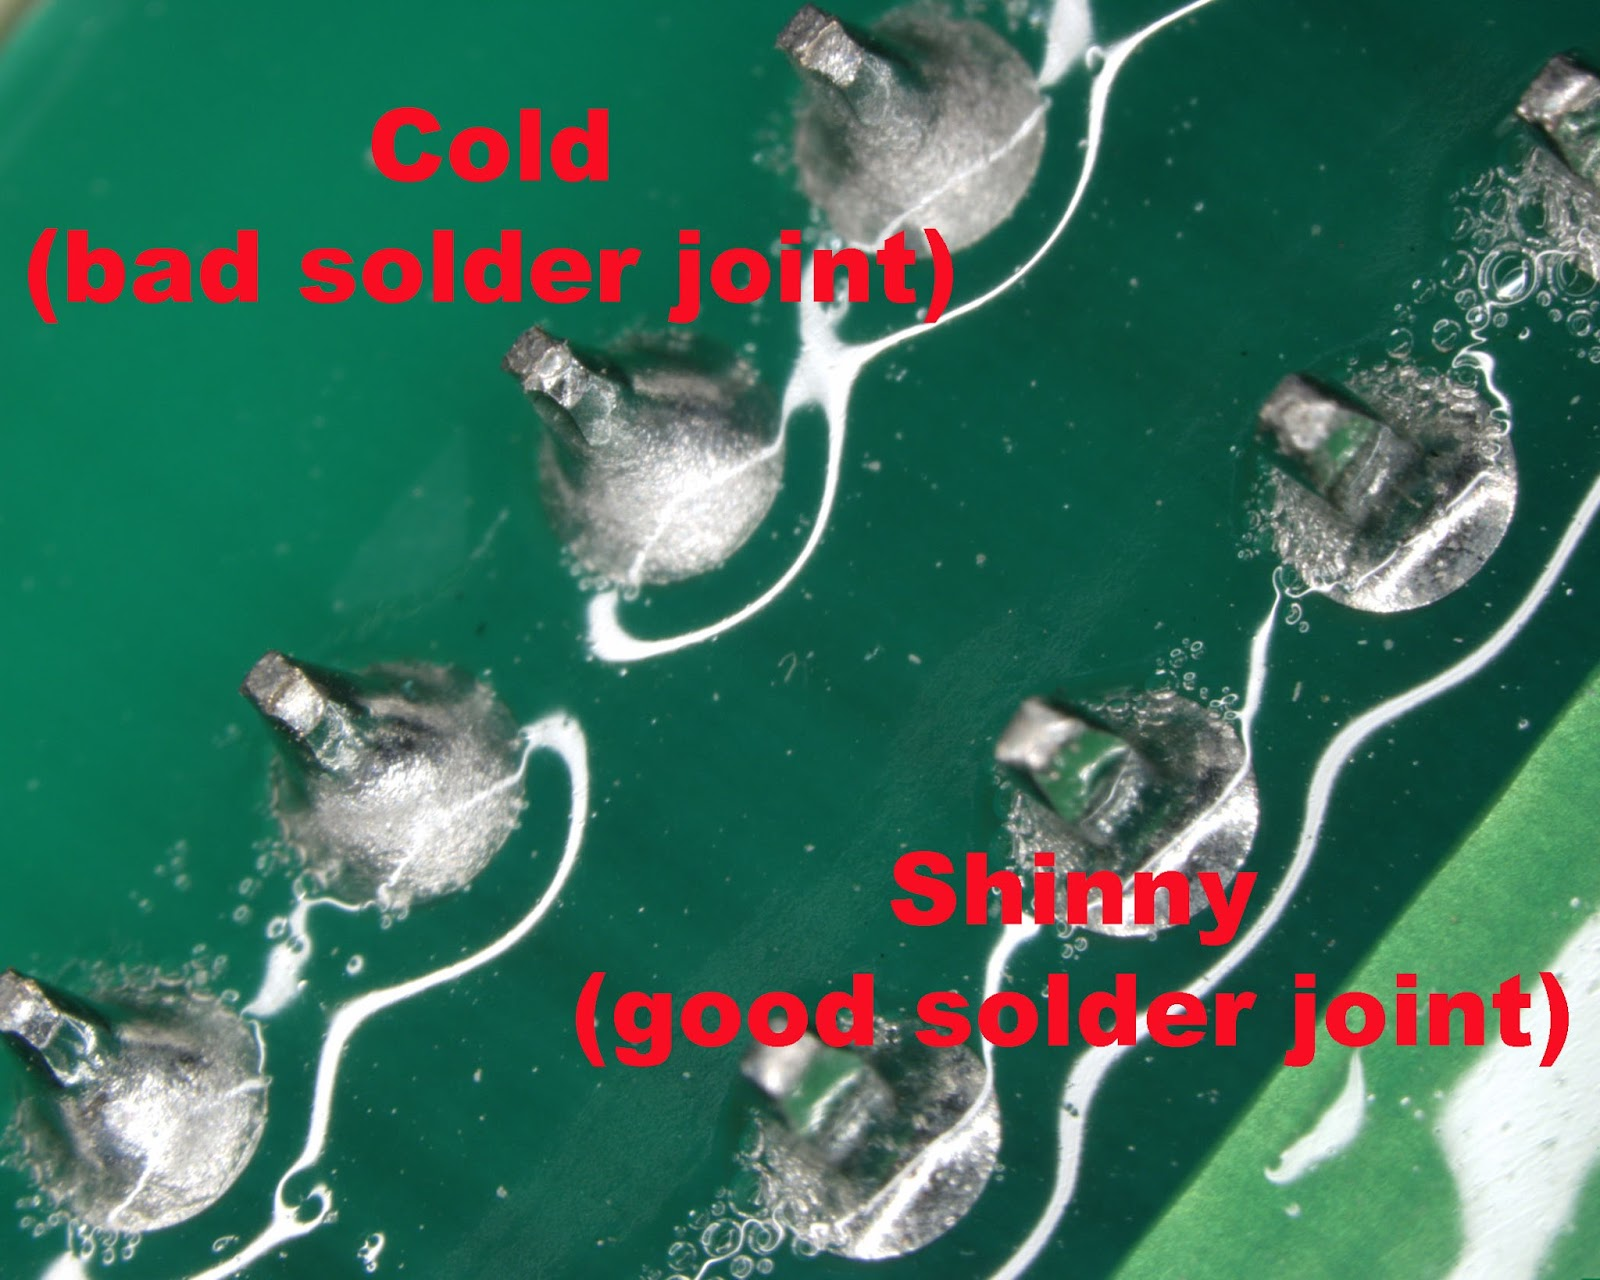
\includegraphics[scale=0.25]{images/joints.jpg}
\end{figure}

\pagebreak

\subsection{Removing Solder}
The best way to remove solder is with solder braid (also called solder wick). Solder braid is a strip of thin copper wires braided together and coated in flux, and is specifically designed to wick away excess solder.
\begin{enumerate}
    \item Coat the tip in a little solder.
    \item Place the braid between the tip and the joint, then press the tip firmly onto the braid covering the joint. Wait until the joint melts and the wick absorbs the excess solder.
    \item Move the iron and the braid away at the same time. Otherwise, the braid will become stuck to the joint.
    \item Re-solder the joint and be sure to use less solder than before.
\end{enumerate}
\begin{figure}[h]
    \caption{removing solder from a joint using solder braid.}
    \centering 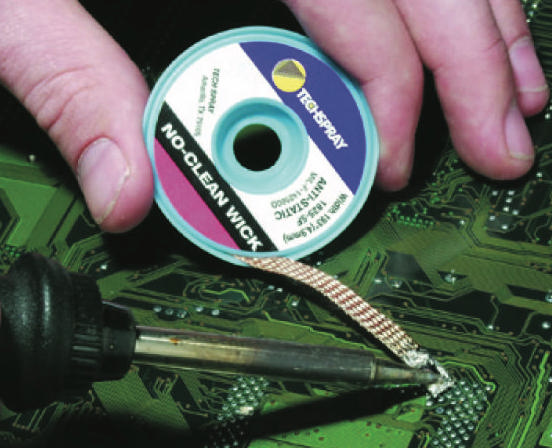
\includegraphics[scale=0.5]{images/wicking.jpg}
\end{figure}

\noindent The following sections contain hyperlinks. If these do not work, download the PDF and open it with a PDF viewer. Do not use GitHub's PDF viewer.

\section{Additional Resources}
\href{https://docs.google.com/presentation/d/1gsUb53UJUmAFMdqCDinAuhG2tvJvpA0dKFnbgJBPr4M/edit?usp=sharing}{Slideshow with additional images} \\
\href{https://www.youtube.com/watch?v=VxMV6wGS3NY}{Video demonstrating how to solder}

\section{Image Sources}
\href{https://www.pinterest.com/pin/250g-multicore-solder-38mm015-diameter-6337-370-flux-5core-mm01082--410672059781838162/}{Figure 1} \\
\href{https://scienceprog.com/reliable-soldering-with-fluxes/}{Figure 2} \\
\href{https://www.amazon.com/Solder-Flux-Paste-grams-ounces/dp/B09DDCNJS9}{Figure 3 [a]}, 
\href{https://www.amazon.com/Chipquik-Tack-clean-syringe-plunger/dp/B00CM2A97S}{Figure 3 [b]}, 
\href{https://www.kester.com/products/product/951-flux-pen}{Figure 3 [c]} \\
\href{https://kb.hakkousa.com/Knowledgebase/10322/How-to-Maximize-Soldering-Iron-Tip-Life}{Figure 4} \\
\href{https://hakkousa.com/599b-tip-cleaner.html}{Figure 5} \\
\href{https://www.hakko.com/english/support/maintenance/detail.php?seq=183}{Figure 6} \\
\href{https://hakkousa.com/t18-d16-chisel-tip.html}{Figure 7[a]}, 
\href{https://hakkousa.com/t18-b-conical-tip.html}{Figure 7 [b]} \\
\href{https://llllllll.co/t/soldering-qs/3757}{Figure 8} \\
\href{https://www.newark.com/techspray/1821-10f/desoldering-braid/dp/69K7664}{Figure 9}
\end{document}
